\documentclass{article}

\usepackage{neurips_2022}
\usepackage[utf8]{inputenc}
\usepackage[T1]{fontenc}
\usepackage{hyperref}
\usepackage{url}
\usepackage{booktabs}
\usepackage{amsfonts}
\usepackage{nicefrac}
\usepackage{microtype}
\usepackage{xcolor}
\usepackage{amsmath}
\usepackage{amssymb}
\usepackage[UTF8, fontset=adobe]{ctex}
\usepackage{algorithm}
\usepackage{algpseudocode}
\usepackage{resizegather}
\usepackage{graphicx}
\usepackage{subfigure}

\hypersetup{
    colorlinks=true,
    linkbordercolor=white
}
\setlength{\parindent}{2em}

\title{数值代数大作业报告}

\author{
    陈润璘 \\
    \texttt{2200010848}
}

\begin{document}

\maketitle

\section{问题描述}

\subsection{Stokes 方程}

Stokes 方程

\begin{equation*}
    \begin{cases}
        -\Delta \vec{u} + \nabla p = \vec{F}, & (x,y)\in (0,1)\times (0,1), \\
        \textrm{div}\, \vec{u} = 0, & (x,y)\in (0,1)\times (0,1), \\
    \end{cases}
\end{equation*}

是一个二维的不可压缩流体的流动方程。其中 $\vec{u} = (u,v)$ 表示速度,$p$ 表示压力,$\vec{F}$ 表示外力。

在本次大作业中,我们考虑如下的边值条件:

\begin{equation*}
    \begin{aligned}
        &\frac{\partial u}{\partial \vec{n}}=b, y=0,\quad \frac{\partial u}{\partial \vec{n}}=t, y=1\\
        &\frac{\partial v}{\partial \vec{n}}=l, x=0,\quad \frac{\partial v}{\partial \vec{n}}=r, x=1\\
        & u=0, x = 0, 1,\quad v=0, y = 0, 1
    \end{aligned}
\end{equation*}

\subsection{交错网格上的 MAC 格式}

根据方程的结构,可以设计出一个交错网格上的离散格式。我们将速度和压力分别定义在交错网格上,其中速度定义在相邻格点连线的中点上,压力定义在每个网格的中心。我们用 $u_{i,j}, v_{i,j}, p_{i,j}$ 分别表示离散后的速度和压力。使用有限差分近似原方程,即可得到如下的线性方程组:

\begin{equation*}
    \begin{pmatrix}
        A & B \\
        B^T & 0
    \end{pmatrix}
    \begin{pmatrix}
        U \\
        P
    \end{pmatrix}
    =
    \begin{pmatrix}
        F \\
        0
    \end{pmatrix}
\end{equation*}

其中 $A =
\begin{pmatrix}
    A_u & 0 \\
    0 & A_v
\end{pmatrix}$
$B =
\begin{pmatrix}
    B_u \\ B_v
\end{pmatrix}$

\begin{equation*}
    \begin{aligned}
        & A_u =
        \begin{pmatrix}
            A_1 & -\frac{1}{h^2} I & &\\
            -\frac{1}{h^2} I & A_2 & -\frac{1}{h^2} I\\
            & \ddots & \ddots & \ddots\\
            & & -\frac{1}{h^2} I & A_2 & -\frac{1}{h^2} I\\
            & & & -\frac{1}{h^2} I & A_1
        \end{pmatrix},
        A_v =
        \begin{pmatrix}
            A_3 & -\frac{1}{h^2} I & &\\
            -\frac{1}{h^2} I & A_3 & -\frac{1}{h^2} I\\
            & \ddots & \ddots & \ddots\\
            & & -\frac{1}{h^2} I & A_3 & -\frac{1}{h^2} I\\
            & & & -\frac{1}{h^2} I & A_3
        \end{pmatrix}, \\
        & A_1 =
        \begin{pmatrix}
            \frac{3}{h^2} & -\frac{1}{h^2} \\
            -\frac{1}{h^2} & \frac{3}{h^2} & -\frac{1}{h^2} \\
            & \ddots & \ddots &\ddots \\
            && -\frac{1}{h^2} & \frac{3}{h^2} & -\frac{1}{h^2} \\
            &&& -\frac{1}{h^2} & \frac{3}{h^2}
        \end{pmatrix}, A_2 =
        \begin{pmatrix}
            \frac{4}{h^2} & -\frac{1}{h^2} \\
            -\frac{1}{h^2} & \frac{4}{h^2} & -\frac{1}{h^2} \\
            & \ddots & \ddots &\ddots \\
            && -\frac{1}{h^2} & \frac{4}{h^2} & -\frac{1}{h^2} \\
            &&& -\frac{1}{h^2} & \frac{4}{h^2}
        \end{pmatrix}, \\
        & A_3 =
        \begin{pmatrix}
            \frac{3}{h^2} & -\frac{1}{h^2} \\
            -\frac{1}{h^2} & \frac{4}{h^2} & -\frac{1}{h^2} \\
            & \ddots & \ddots &\ddots \\
            && -\frac{1}{h^2} & \frac{4}{h^2} & -\frac{1}{h^2} \\
            &&& -\frac{1}{h^2} & \frac{3}{h^2}
        \end{pmatrix}, \\
        & B_u =
        \begin{pmatrix}
            H \\
            & H \\
            & & \ddots \\
            & & & H
        \end{pmatrix},
        B_v =
        \begin{pmatrix}
            -\frac{1}{h} I_{N\times N} & \frac{1}{h} I_{N\times N} \\
            & -\frac{1}{h} I_{N\times N} & \frac{1}{h} I_{N\times N} \\
            & & \ddots & \ddots \\
            & & & -\frac{1}{h} I_{N\times N} & \frac{1}{h} I_{N\times N}
        \end{pmatrix}, \\
        & H =
        \begin{pmatrix}
            -\frac{1}{h} & \frac{1}{h}\\
            & -\frac{1}{h} & \frac{1}{h} \\
            & & \ddots & \ddots \\
            & & & -\frac{1}{h} & \frac{1}{h} \\
        \end{pmatrix}
    \end{aligned}
\end{equation*}

上述矩阵中,$A_u,A_v$ 均为 $N(N-1)\times N(N-1)$ 的矩阵,$A_1, A_2$ 为 $(N-1)\times(N-1)$ 的矩阵,$A_3$ 为 $N\times N$ 的矩阵,$H$ 为 $(N-1)\times N$ 的矩阵。

\subsection{数值算例}

在本次作业中我们考虑如下的数值算例:

\begin{equation*}
    \begin{aligned}
        & f(x,y)=4\pi^2(2\cos(2\pi x)-1)\sin(2\pi y)+x^2 \\
        & g(x,y)=4\pi^2(2\cos(2\pi y)-1)\sin(2\pi x)
    \end{aligned}
\end{equation*}

在以上的压力条件下,Stokes 方程的真解为

\begin{equation*}
    \begin{aligned}
        & u(x,y)=(1-\cos(2\pi x))\sin(2\pi y) \\
        & v(x,y)=-(1-\cos(2\pi y))\sin(2\pi x) \\
        & p(x,y)=\frac{x^3}{3} - \frac{1}{12}
    \end{aligned}
\end{equation*}

我们将使用多重网格方法求解 1.2 中的线性方程组,并对比与真解之间的误差。

\section{数值方法}

\subsection{以 DGS 为磨光子的 V-cycle 多重网格方法}

Distributive Gauss-Seidel (DGS) 迭代法的一次迭代中先处理第一个方程 $AU+BP=F$,将其改写为 $AU=F-BP$,使用 Gauss-Seidel 迭代法更新一次 $U$。然后再考虑散度方程,对每个点依次计算其散度残量
\begin{equation*}
    r_{i,j} = -\frac{u_{i,j-\frac{1}{2}}-u_{i-1,j-\frac{1}{2}}}{h} - \frac{v_{i-\frac{1}{2},j}-v_{i-\frac{1}{2},j-1}}{h}
\end{equation*}
并根据它更新速度和压力。

在使用 DGS 迭代若干次后,我们计算其误差,并将误差限制在粗网格上继续迭代。由于 DGS 迭代具有魔光性,误差的高频部分已经消失,粗网格上的限制可以较好地近似低频的误差。在粗网格上迭代若干此后在将误差限制在更粗的网格上,不断这样进行直到最粗的网格上。在最粗的网格上迭代若干次后,我们将校正量提升回细网格上,并使用 DGS 迭代法迭代若干此。由于每一次限制后方程组的阶数都除以 4,因此一次 V-cycle 迭代的主要计算量都在最细的网格上。

\subsection{Uzawa 迭代法}

Uzawa 迭代法的迭代格式如下:

\begin{itemize}
    \item 求解速度方程 $AU_{k+1}=F-BP_{k}$。
    \item 更新压力 $P_{k+1}=P_{k}+\alpha B^T U_{k+1}$。
    \item 判断是否收敛,若未收敛则继续迭代。
\end{itemize}

在求解速度方程时,由于矩阵 $A$ 是对称正定的,我们可以使用 LDL 分解或共轭梯度法求解。在更新压力时,每一次迭代可以写成如下的形式:

\begin{equation*}
    \begin{aligned}
        P_{k+1} &= P_{k} + \alpha B^T U_{k+1} \\
        &= P_{k} + \alpha B^T A^{-1} (F-BP_{k}) \\
        &= (I-\alpha B^T A^{-1} B)P_{k} + \alpha B^T A^{-1} F
    \end{aligned}
\end{equation*}

这相当于使用迭代法求解线性方程组 $B^T A^{-1} B P = B^T A^{-1} F$,因而应当取 $\alpha$ 使得 $I-\alpha B^T A^{-1} B$ 的谱半径最小。在实现算法时,我们取 $\alpha=1$。

\subsection{Inexact Uzawa 迭代法}

在使用 Uzawa 迭代法时,虽然只用很少的迭代次数就能达到很小的误差,但是每一次迭代都需要求解一个线性方程组,这是一个很大的计算量。因此我们可以使用 Inexact Uzawa 迭代法,即在求解速度方程时只求解一个近似解,而不是精确解。在求解速度方程时,我们可以使用预优共轭梯度法求解,这样可以大大减少计算量,加快求解速度。

预优共轭梯度法的迭代格式如下:
\begin{algorithm}
    \caption{预优共轭梯度法}
    \begin{algorithmic}
        \State $k \gets 0$, r $\gets b-Ax$, $\rho=r^T r$
        \While{$\sqrt{r^T r}>\max(\epsilon\|b\|_2, \tau \|B^T U_k\|)$ and $k<k_{\max}$}
        \State $k \gets k+1$
        \State 使用 V-cycle 多重网格法近似求解 $Az = r$
        \If{$k=1$}
        \State $p \gets z$, $\rho \gets r^T z$
        \Else
        \State $\rho' \gets \rho$, $\rho \gets r^T z$, $\beta \gets \rho/\rho'$, $p \gets z+\beta p$
        \EndIf
        \State $w \gets Ap$, $\alpha \gets \rho/(p^T w)$, $x \gets x+\alpha p$, $r \gets r-\alpha w$
        \EndWhile
    \end{algorithmic}
    \label{alg:pcg}
\end{algorithm}
\newline
在使用多重网格法近似求解 $Az=r$ 时,只需迭代几步即可,不用精确求解。

\section{算法实现}

\subsection{在 CPU 上算法实现}

由于上述的三种算法在实现时难以利用已有的线性代数库中提供的函数,因此为了保证算法的效率,我们使用 C++ 语言和 Eigen 库实现了这三种算法。

在实现这三种算法时,可以利用 CPU 的多个核心进行并行计算,提高计算效率。在使用 Gauss-Seidel 迭代法时,由于 $u,v$ 的更新互不影响,因此可以将他们分配到两个线程上并行计算。在 DGS 迭代更新压力时,如图 \ref{fig:split} 所示,可以将压力矩阵 $P$ 分为若干部分,首先并行地更新标号为 1 的四个部分,再并行地更新标号为 2 的四个部分,最后更新标号为 3 的 4 各单元。

\begin{figure}
    \centering
    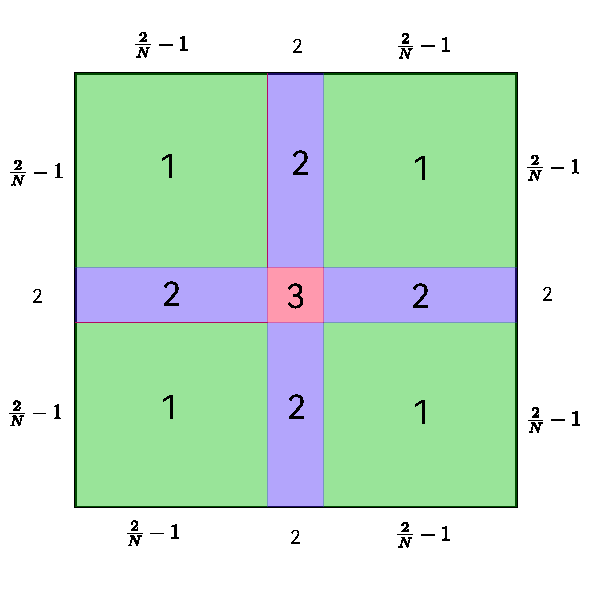
\includegraphics[width=0.4\textwidth]{fig/split.pdf}
    \caption{将压力矩阵 $P$ 按照 4 个部分}
    \label{fig:split}
\end{figure}

\subsection{在 GPU 上算法实现}

GPU 的并行计算能力远远超过 CPU,因此我们可以利用 GPU 的高并行度进一步提高算法的效率。在本次大作业中,我使用 \href{https://triton-lang.org/main/index.html}{Triton} 实现 V-cycle 多重网格法。

在进行 Gauss-Seidel 迭代更新 $u$ 时,可以先并行地更新所有奇数行,再并行地更新所有偶数行,更新 $v$ 时,可以先并行地更新所有奇数列,再并行地更新所有偶数列。在更新压力时,可以将压力矩阵 $P$ 按照行序号 $\mod 4$ 的余数分为 4 个部分,每一次并行地更新每一部分。

\section{数值结果}

\subsection{V-cycle 多重网格法}

在 CPU 上实现的 V-cycle 多重网格法的数值结果如下:

\begin{table}[H]
    \centering
    \resizebox{\textwidth}{!}{
        \begin{tabular}{c|ccccccc}
            \toprule
            \hline
            N & 64 & 128 & 256 & 512 & 1024 & 2048 & 4096 \\
            \hline
            时间 (s) & 0.009894 & 0.024583 & 0.070604 & 0.254675 & 0.933841 & 3.312589 & 14.814826 \\
            \hline
            迭代次数 & 7 & 7 & 7 & 7 & 7 & 6 & 6 \\
            \hline
            误差 & 1.495079e-03 & 3.736293e-04 & 9.339865e-05 & 2.334926e-05 & 5.837405e-06 & 1.466171e-06 & 3.753824e-07 \\
            \hline
            \bottomrule
        \end{tabular}
    }
    \caption{V-cycle 多重网格法在 CPU 上的数值结果}
    \label{tab:v-cycle-cpu}
\end{table}

在 GPU 上实现的 V-cycle 多重网格法的数值结果如下:

\begin{table}[H]
    \centering
    \resizebox{\textwidth}{!}{
        \begin{tabular}{c|ccccccc}
            \toprule
            \hline
            N & 64 & 128 & 256 & 512 & 1024 & 2048 & 4096 \\
            \hline
            时间 (s) & 0.050207 & 0.066984 & 0.113088 & 0.202515 & 0.405535 & 0.941348 & 2.450048 \\
            \hline
            迭代次数 & 10 & 9 & 9 & 9 & 9 & 9 & 9 \\
            \hline
            误差 & 1.495078e-03 & 3.736265e-04 & 9.339932e-05 & 2.335376e-05 & 5.850935e-06 & 1.505012e-06 & 5.105759e-07 \\
            \hline
            \bottomrule
        \end{tabular}
    }
    \caption{V-cycle 多重网格法在 GPU 上的数值结果}
    \label{tab:v-cycle-gpu}
\end{table}

其中 N 为横纵方向分点的数目,误差使用以下的公式计算:
\begin{equation*}
    e_N = h\left(\sum_{j=1}^{N}\sum_{i=1}^{N-1}\left|u_{i,j-\frac{1}{2}}-u(x_i,y_{j-\frac{1}{2}})\right|^2 +
    \sum_{j=1}^{N-1}\sum_{i=1}^{N}\left|v_{i-\frac{1}{2},j}-v(x_{i-\frac{1}{2}},y_{j})\right|^2\right)^{\frac{1}{2}}
\end{equation*}

由表 \ref{tab:v-cycle-cpu} 和表 \ref{tab:v-cycle-gpu} 可以看出,在分点数较多时,GPU 上的并行算法的求解速度远超 CPU 上的算法,在 $N=2048$ 或 $4096$ 时,GPU 上的算法的求解速度能提升 3-6 倍。但是,由于 GPU 上的并行 DGS 迭代算法的磨光性较差,因此在迭代次数上 GPU 上的算法比 CPU 上的算法多。

\begin{figure}[H]
    \centering
    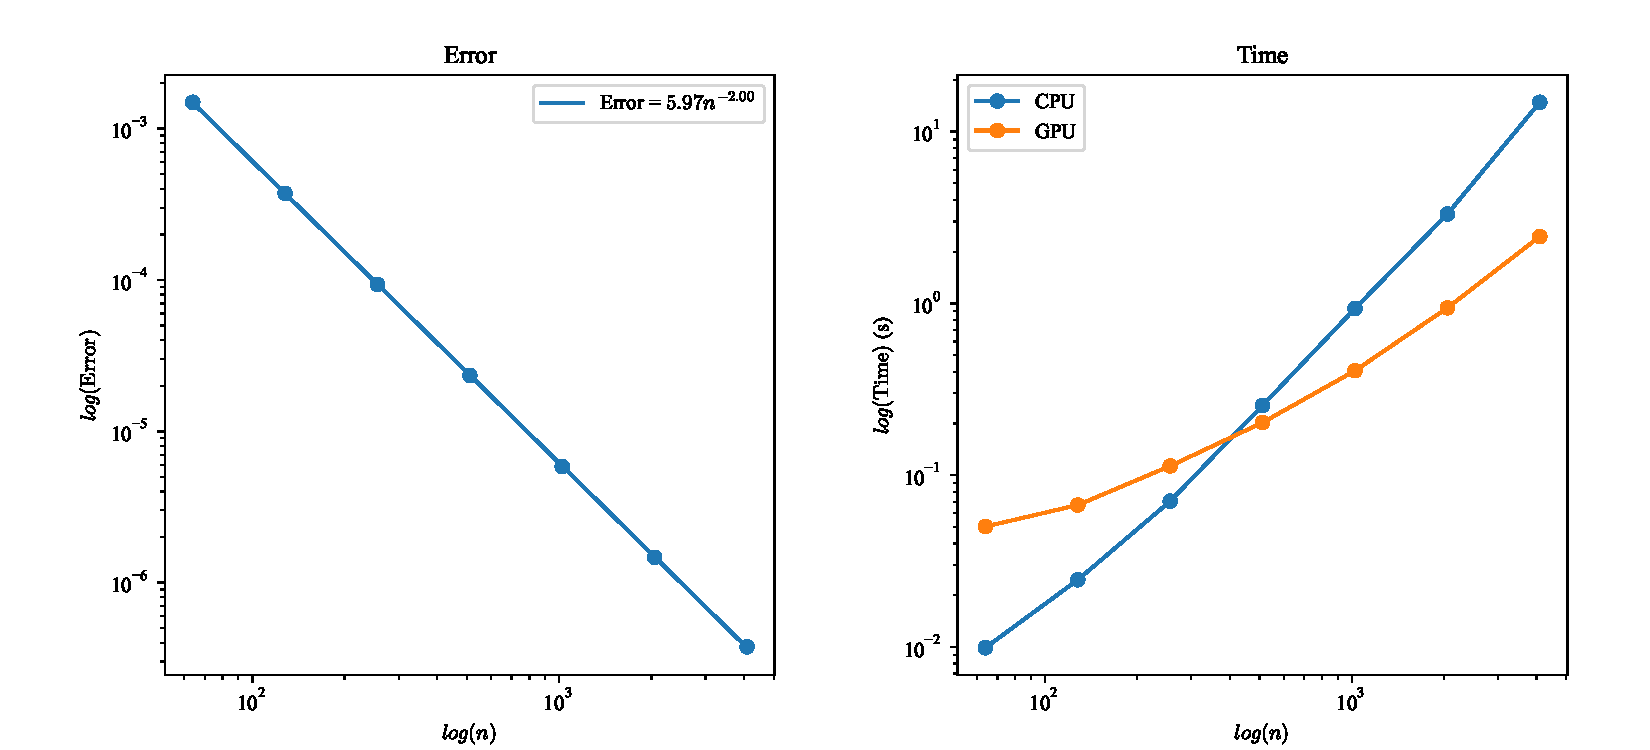
\includegraphics[width=\textwidth]{fig/vcycle.pdf}
    \caption{V-cycle 多重网格法的误差和时间随分点数变化的图像}
    \label{fig:vcycle}
\end{figure}

图 \ref{fig:vcycle} 展示了 V-cycle 多重网格法的误差和时间随分点数变化的图像。从图中可以看出,误差与分点数 $N$ 的平方成反比,即 $e_N\propto N^{-2}$;在 GPU 上的算法的时间的增长速度比 CPU 上的算法慢得多。

\subsection{Uzawa 迭代法和 Inexact Uzawa 迭代法}

Uzawa 迭代法和 Inexact Uzawa 迭代法的数值结果如下:

\begin{table}[H]
    \centering
    \resizebox{0.7\textwidth}{!}{
        \begin{tabular}{c|cccc}
            \toprule
            \hline
            N & 64 & 128 & 256 & 512 \\
            \hline
            时间 (s) & 0.013037 & 0.052010 & 0.297795 & 2.441135 \\
            \hline
            迭代次数 & 2 & 2 & 2 & 2 \\
            \hline
            误差 & 1.495079e-03 & 3.736291e-04 & 9.339849e-05 & 2.334907e-05 \\
            \hline
            \bottomrule
        \end{tabular}
    }
    \caption{Uzawa 迭代法的数值结果}
    \label{tab:uzawa}
\end{table}

\begin{table}[H]
    \centering
    \resizebox{\textwidth}{!}{
        \begin{tabular}{c|cccccc}
            \toprule
            \hline
            N & 64 & 128 & 256 & 512 & 1024 & 2048 \\
            \hline
            时间 (s) & 0.012122 & 0.031504 & 0.117809 & 0.424421 & 1.637968 & 6.906212 \\
            \hline
            迭代次数 & 2 & 2 & 2 & 2 & 2 & 2 \\
            \hline
            误差 & 1.495079e-03 & 3.736292e-04 & 9.339860e-05 & 2.334917e-05 & 5.837325e-06 & 1.459394e-06 \\
            \hline
            \bottomrule
        \end{tabular}
    }
    \caption{Inexact Uzawa 迭代法的数值结果}
    \label{tab:inexact-uzawa}
\end{table}

对比表 \ref{tab:uzawa} 和表 \ref{tab:inexact-uzawa} 的结果不难发现,以 V-cycle 多重网格法为预条件子的预优共轭梯度法的求解速度明显快于普通的共轭梯度法,这使得 Uzawa 迭代法能够求解更大规模的问题。但是,由于 Inexact Uzawa 迭代法每一次迭代都需要求解一个线性方程组,因此其求解速度仍然慢于 V-cycle 多重网格法。

\begin{figure}[H]
    \centering
    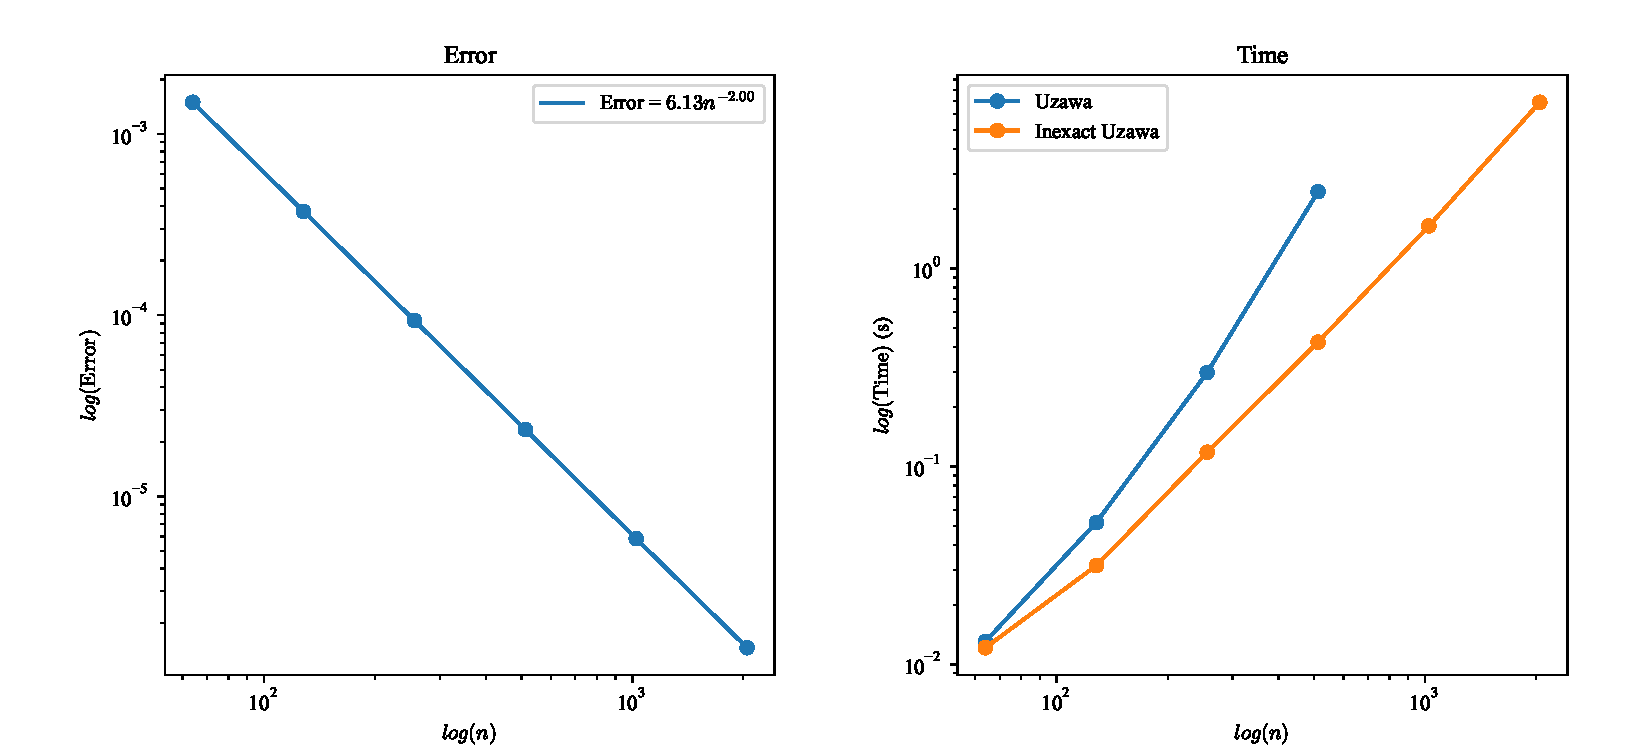
\includegraphics[width=\textwidth]{fig/uzawa.pdf}
    \caption{Uzawa 迭代法和 Inexact Uzawa 迭代法的误差和时间随分点数变化的图像}
    \label{fig:uzawa}
\end{figure}

图 \ref{fig:uzawa} 展示了 Uzawa 迭代法和 Inexact Uzawa 迭代法的误差和时间随分点数变化的图像。与 V-cycle 多重网格法相同,Inexact Uzawa 迭代法的误差也与 $N$ 的平方成反比。与直接使用共轭梯度法求解速度方程的 Uzawa 迭代法相比,使用了预优共轭梯度法的 Inexact Uzawa 迭代法的用时随分点数 $N$ 的增长速度远慢于 Uzawa 迭代法。

\end{document}
